\chapter{Heat and Insulation}\label{ch:g5:heat-and-insulation}

Why does the metal slide feel icy when the wooden bench beside it
does not? That mystery has trailed us since the first year of this
book. Today it falls --- together with the secrets of the thermos,
the double window, and the puffed-up winter sparrow. The key is to
stop asking how things \emph{feel} and start following where \omterm{def:g5:heat-and-insulation:heat}{heat}
\emph{flows}.

\section{Heat is on the move}

\begin{definition}[Heat]\label{def:g5:heat-and-insulation:heat}
\emph{Heat}\index{heat} is \omterm{def:g5:everyday-energy:energy}{energy} on the move from a hotter thing
to a colder one. The soup passes heat to the spoon, the radiator to
the room, your hand to a snowball. Heat is not a stuff hiding
inside hot things --- it is a \emph{flow}, and it always has a
direction.
\end{definition}

\begin{proposition}[Heat flows downhill]\label{prop:g5:heat-and-insulation:downhill}
By itself, \omterm{def:g5:heat-and-insulation:heat}{heat} always flows from the hotter body to the colder
one --- never the other way. The flow runs as long as the two
\omterm{def:g3:temperature-thermometers:temperature}{temperatures} differ, and dies away as they meet: left together
long enough, hot and cold neighbors end up at one shared
\omterm{def:g3:temperature-thermometers:temperature}{temperature}.
\end{proposition}

\begin{example}[Reading the direction]\label{ex:g5:heat-and-insulation:direction}
The teaspoon in the tea grows hot: \omterm{def:g5:heat-and-insulation:heat}{heat} flowed tea $\to$ spoon.
The lemonade with ice grows cold --- careful! Nothing called
``cold'' flowed in: \omterm{def:g5:heat-and-insulation:heat}{heat} flowed \emph{out of the lemonade into the
ice}, melting it. Cold is not a flow; it is only the name we give
the loser's side. Physics books all say ``the drink loses \omterm{def:g5:heat-and-insulation:heat}{heat}'',
never ``the drink gains cold''.
\end{example}

\begin{omfigure}
\begin{tikzpicture}[scale=0.85]
  \draw[thick] (0.6,0.4) rectangle (3.0,1.9);
  \node[font=\small] at (1.8,1.15) {hot soup};
  \draw[thick] (7.8,0.4) rectangle (10.2,1.9);
  \node[font=\small] at (9.0,1.15) {cool air};
  \draw[-Stealth, line width=3pt, omThm] (3.3,1.15) -- (7.5,1.15);
  \node[above, font=\small, omThm] at (5.4,1.4)
    {heat flows hot $\to$ cold};
  \node[below, font=\small] at (5.4,0.0)
    {and stops only when the two temperatures meet};
\end{tikzpicture}

{\small One rule for every kitchen and every winter: \omterm{def:g5:heat-and-insulation:heat}{heat} runs
downhill, from hotter to colder, until the hill is gone.}
\end{omfigure}

\section{Fast lanes and slow lanes}

\begin{definition}[Heat conductors and insulators]\label{def:g5:heat-and-insulation:conductors}
Stuffs differ wildly in how fast they let \omterm{def:g5:heat-and-insulation:heat}{heat} flow through them. A
\emph{heat conductor}\index{heat conductor} is a fast lane ---
metals above all. A \emph{heat insulator}\index{heat insulator} is
a slow lane: wood, wool, plastic, feathers --- and the champion,
\emph{still \omterm{def:g2:air-around-us:air}{air}}, trapped so it cannot swirl. (The words are
borrowed on purpose from electricity's \omterm{def:g4:conductors-insulators:conductor}{conductors} and \omterm{def:g4:conductors-insulators:insulator}{insulators};
the two properties often, but not always, go together.)
\end{definition}

\begin{omfigure}
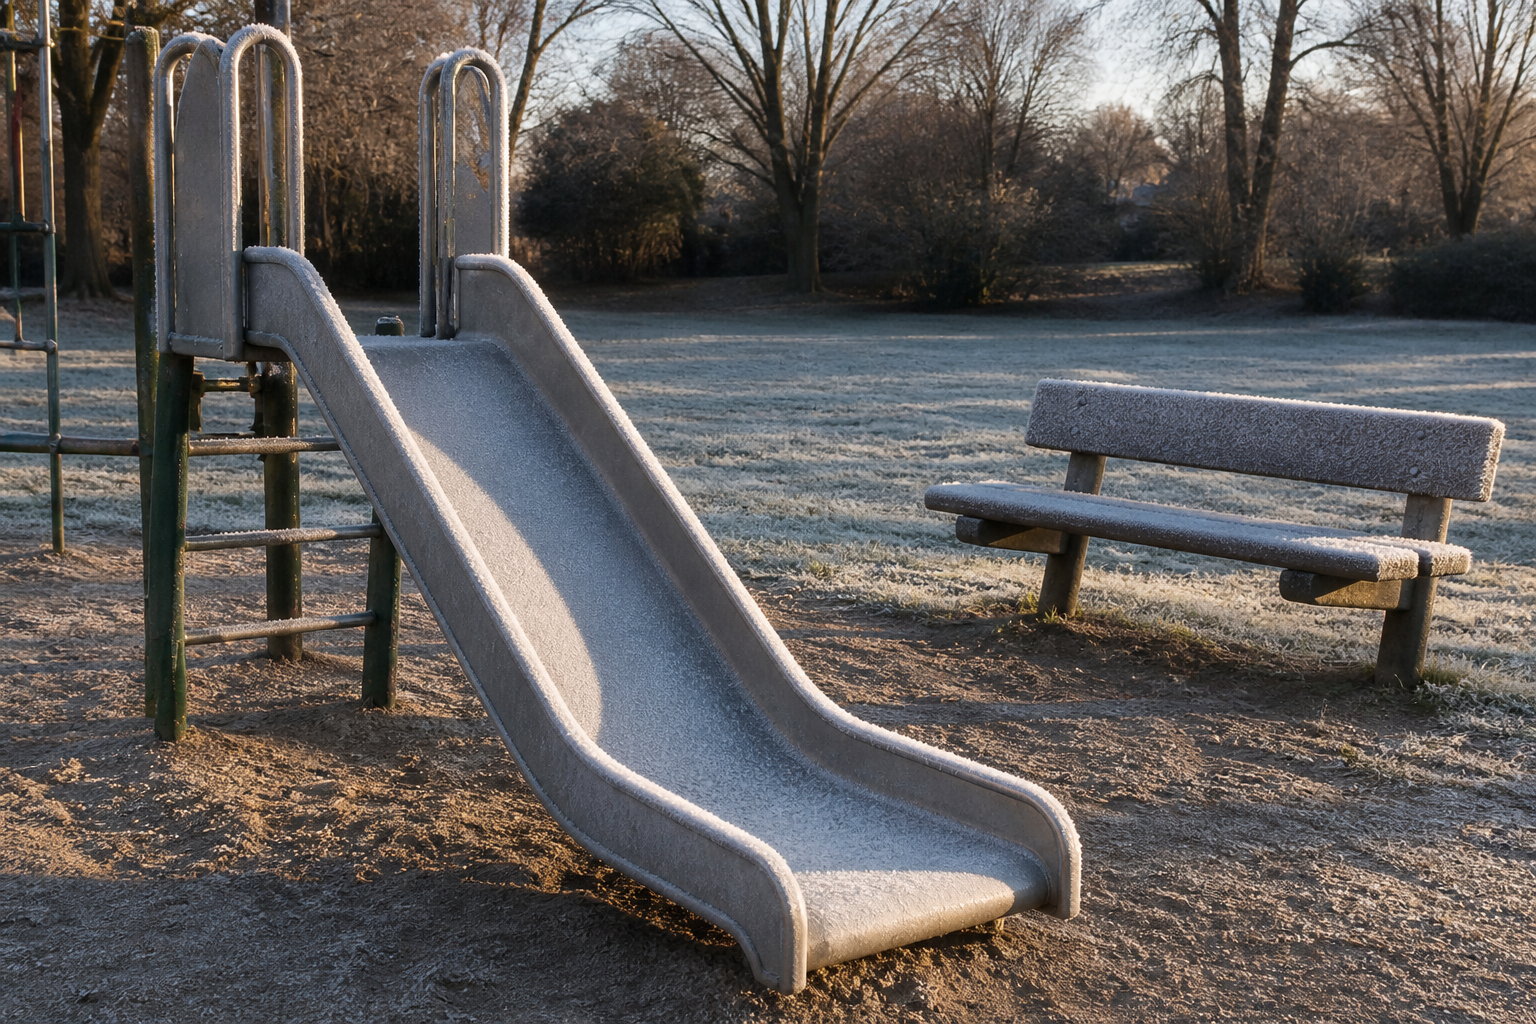
\includegraphics[width=0.58\linewidth]{images/book1/ai/g5-heat-frosty-slide.png}

{\small A frosty morning on the playground: metal slide and wooden bench spent the same night at the same \omterm{def:g3:temperature-thermometers:temperature}{temperature} --- yet only one of them will bite your skin.}
\end{omfigure}

\begin{example}[The slide mystery, solved]\label{ex:g5:heat-and-insulation:slide}
The metal slide and the wooden bench spent the night at the same
chilly \omterm{def:g3:temperature-thermometers:temperature}{temperature} --- the \omterm{def:g3:temperature-thermometers:temperature}{thermometer} swore it long ago. Touch
them: your hand is warmer than both, so \omterm{def:g5:heat-and-insulation:heat}{heat} flows from you into
each. But the metal is a fast lane --- it whisks your \omterm{def:g5:heat-and-insulation:heat}{heat} away in
a rush, and that \emph{rush} is what ``icy'' feels like. The wood
takes your \omterm{def:g5:heat-and-insulation:heat}{heat} only in a trickle: barely cool. Your skin was
never measuring \omterm{def:g3:temperature-thermometers:temperature}{temperature} --- it \omterm{def:g2:measuring-length:measure}{measures} the speed of its own
\omterm{def:g5:heat-and-insulation:heat}{heat} loss. Case closed, after four years.
\end{example}

\begin{method}[The cooling race]\label{met:g5:heat-and-insulation:race}
Watch insulation win, with numbers:
\begin{enumerate}
  \item fill two identical mugs with equally hot tap water
        (\emph{ask an adult for hand-hot, not boiling});
  \item wrap one mug thickly in a wool scarf; leave the other bare;
  \item plant a \omterm{def:g3:temperature-thermometers:temperature}{thermometer} in each and write both \omterm{def:g3:temperature-thermometers:temperature}{temperatures} in
        a table every five minutes, six times;
  \item draw both records as two lines on one graph, \omterm{def:g3:temperature-thermometers:temperature}{temperature}
        against time.
\end{enumerate}
The bare mug's line dives; the wrapped mug's line slopes gently.
Same start, same room --- the wool made \omterm{def:g5:heat-and-insulation:heat}{heat}'s exit a slow lane.
\end{method}

\begin{omfigure}
\begin{tikzpicture}
\begin{axis}[omaxis, width=10.5cm, height=5.6cm,
    xlabel={minutes}, ylabel={temperature (\unit{\celsius})},
    xtick={0,5,10,15,20,25,30}, ytick={20,30,40,50},
    ymin=15, ymax=55, xmin=-1, xmax=31]
  \addplot[very thick, omDef] coordinates
    {(0,50) (5,46.5) (10,43.5) (15,41) (20,39) (25,37.5) (30,36)};
  \addplot[very thick, omThm] coordinates
    {(0,50) (5,41) (10,34.5) (15,30) (20,27) (25,24.5) (30,23)};
  \node[right, font=\small, omDef] at (axis cs:24,39.5)
    {wrapped in wool};
  \node[right, font=\small, omThm] at (axis cs:19,25.5) {bare mug};
\end{axis}
\end{tikzpicture}

{\small The cooling race, drawn: two mugs of \qty{50}{\celsius}
water in a \qty{20}{\celsius} room. The wool cannot stop \omterm{def:g5:heat-and-insulation:heat}{heat}'s
escape --- but it slows it beautifully.}
\end{omfigure}

\begin{remark}[Insulation only slows]\label{rem:g5:heat-and-insulation:onlyslows}
Look where both curves are headed: toward the room's
\qty{20}{\celsius}. No scarf, no thermos, no igloo wall ever stops
\omterm{def:g5:heat-and-insulation:heat}{heat}'s downhill flow --- insulation only makes the slow lane
slower. That is also why the coat on the snowman (remember him?)
delayed his melting but could not save him: the summer's \omterm{def:g5:heat-and-insulation:heat}{heat} still
trickled in.
\end{remark}

\section{The art of trapping air}

\begin{example}[Winter engineering]\label{ex:g5:heat-and-insulation:air}
Almost every warm thing you own is a machine for trapping \omterm{def:g2:air-around-us:air}{air}.
Wool keeps you warm not by the fibers themselves but by the
countless \omterm{def:g2:air-around-us:air}{air} pockets between them; feather duvets, fleece and the
sparrow puffed into a ball on a frozen wire all play the same
card. Houses join in: double windows imprison a layer of \omterm{def:g2:air-around-us:air}{air}
between two panes, and insulated walls are filled with fluffy,
air-hoarding padding. Still \omterm{def:g2:air-around-us:air}{air} is the champion slow lane --- the
trick is keeping it \emph{still}.
\end{example}

\begin{example}[The thermos]\label{ex:g5:heat-and-insulation:thermos}
The thermos flask is insulation's masterpiece: a bottle inside a
bottle, with the \omterm{def:g2:air-around-us:air}{air} between them pumped away to almost nothing
--- and where there is almost no stuff, \omterm{def:g5:heat-and-insulation:heat}{heat}'s flow finds almost
no lane at all (a trick worth remembering: the same emptiness that
silenced the bell in the jar). Add shiny walls to bounce warmth's
glow back in, and hot chocolate meets the afternoon still hot ---
or lemonade still cold: the thermos knows nothing of hot or cold,
it only closes the lanes, both ways.
\end{example}

\begin{remark}[Keeping warm, said properly]\label{rem:g5:heat-and-insulation:coat}
Now the old coat question closes for good. A coat is trapped \omterm{def:g2:air-around-us:air}{air}
around a \omterm{def:g5:heat-and-insulation:heat}{heat} maker --- you. Your body streams \omterm{def:g5:heat-and-insulation:heat}{heat} outward all
day; the coat turns that stream into a trickle, and you stay warm
on your own production. On the snowman --- no \omterm{def:g5:heat-and-insulation:heat}{heat} maker inside
--- the same coat merely slows the inward trickle of summer.
Insulation has no favorites: it slows the flow, whichever way it
runs.
\end{remark}

\section{Exercises}

\begin{exercise}[$\star$]\label{exo:g5:heat-and-insulation:1}
What is \omterm{def:g5:heat-and-insulation:heat}{heat}, and in which direction does it flow by itself? When
does the flow stop?
\end{exercise}

\begin{exercise}[$\star$]\label{exo:g5:heat-and-insulation:2}
``Close the door, you are letting the cold in!'' Rewrite
grandmother's sentence the way a physics book would.
\end{exercise}

\begin{exercise}[$\star$]\label{exo:g5:heat-and-insulation:3}
Sort into fast lanes and slow lanes for \omterm{def:g5:heat-and-insulation:heat}{heat}: a copper pan; \ a
wool scarf; \ a steel spoon; \ still \omterm{def:g2:air-around-us:air}{air}; \ a wooden spoon; \ a
duvet.
\end{exercise}

\begin{exercise}[$\star$]\label{exo:g5:heat-and-insulation:4}
Why do pans have metal bottoms but plastic or wooden handles?
Answer with lanes.
\end{exercise}

\begin{exercise}[$\star$]\label{exo:g5:heat-and-insulation:5}
At last, in your own words: why does metal feel colder than wood
at the same \omterm{def:g3:temperature-thermometers:temperature}{temperature}? What does skin really \omterm{def:g2:measuring-length:measure}{measure}?
\end{exercise}

\begin{exercise}[$\star$]\label{exo:g5:heat-and-insulation:6}
In the cooling race, why must the two mugs be identical and start
equally hot? What single difference is the experiment testing?
\end{exercise}

\begin{exercise}[$\star$]\label{exo:g5:heat-and-insulation:7}
Read the cooling graph: about what \omterm{def:g3:temperature-thermometers:temperature}{temperature} is each mug showing
after $15$ minutes? Toward what \omterm{def:g3:temperature-thermometers:temperature}{temperature} are both curves
heading, and why?
\end{exercise}

\begin{exercise}[$\star$]\label{exo:g5:heat-and-insulation:8}
Why does a sparrow puff itself into a ball on a freezing wire?
Name three human inventions playing the same card.
\end{exercise}

\begin{exercise}[$\star\star$]\label{exo:g5:heat-and-insulation:9}
The same thermos keeps chocolate hot in January and lemonade cold
in July. Explain how one device manages both jobs --- what does
the thermos actually do, and to what?
\end{exercise}

\begin{exercise}[$\star\star$]\label{exo:g5:heat-and-insulation:10}
An ice-cream seller wraps her tubs in thick wool blankets on a hot
day, and a customer laughs: ``Wool is for keeping things warm!''
Defend the seller with
\cref{rem:g5:heat-and-insulation:coat} --- which way is \omterm{def:g5:heat-and-insulation:heat}{heat}
trying to flow, and what does the wool do to it?
\end{exercise}

\begin{exercise}[$\star\star$]\label{exo:g5:heat-and-insulation:11}
Two houses stand in the same winter: one with single windows, one
with double windows. Explain with lanes and trapped \omterm{def:g2:air-around-us:air}{air} why the
double-windowed house burns less fuel --- and why, by
\cref{rem:g5:heat-and-insulation:onlyslows}, it still needs
\emph{some} heating.
\end{exercise}
